\documentclass[preprint]{aastex}
\begin{document}
\begin{figure}%[hbt!]
%\centering
\\
\mbox{
          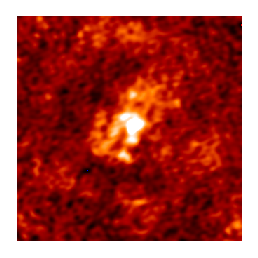
\includegraphics[]{test34.ps}
          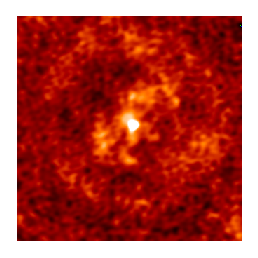
\includegraphics[]{test35.ps}
          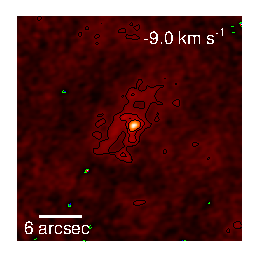
\includegraphics[]{test_34.ps}
          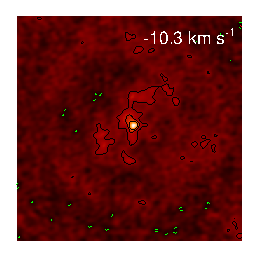
\includegraphics[]{test_35.ps}
          }
\\
\mbox{
          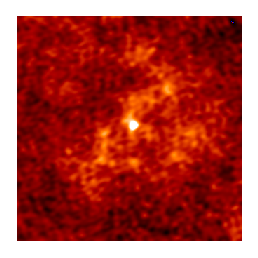
\includegraphics[]{test36.ps}
          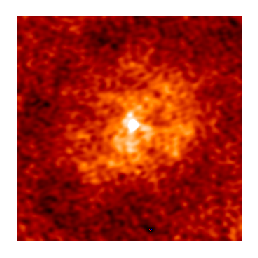
\includegraphics[]{test37.ps}
          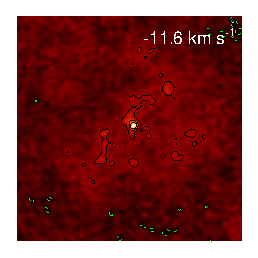
\includegraphics[]{test_36.ps}
          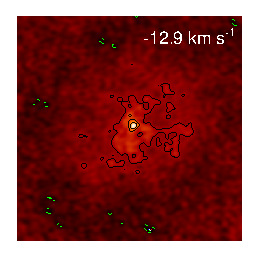
\includegraphics[]{test_37.ps}
          }
\\
\mbox{
          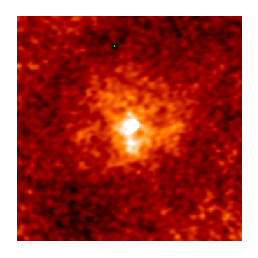
\includegraphics[]{test38.ps}
          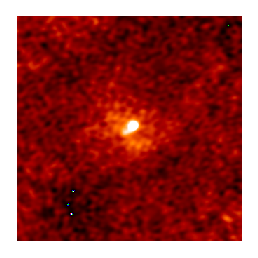
\includegraphics[]{test39.ps}
          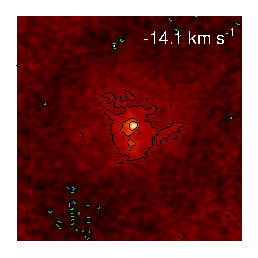
\includegraphics[]{test_38.ps}
          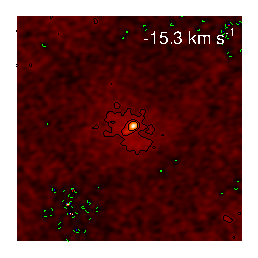
\includegraphics[]{test_39.ps}
          }
\\
\mbox{
          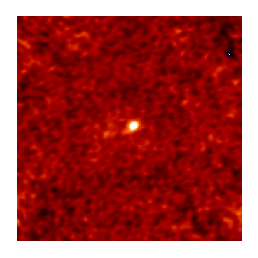
\includegraphics[]{test40.ps}
          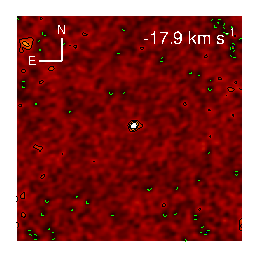
\includegraphics[]{test41.ps}
          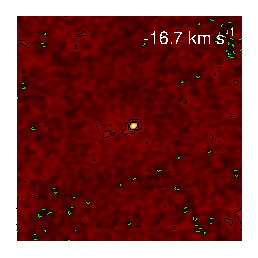
\includegraphics[]{test_40.ps}
          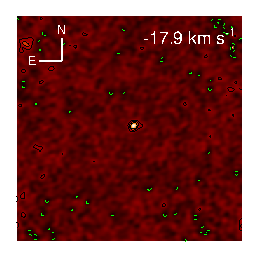
\includegraphics[]{test_41.ps}
          }
          \caption{Channel maps shown in paper (Figure 3) with emission cut at 0.2 Jy beam${}^{-1}$ (left two colums) and with no emission cut off (right two colums).}
\end{figure}

\end{document}